%% Meghan Sullivan
%% 20171205
%% Common factor model

% standalone class for individual image to be included in a document
% border=15pt controls the whitespace padding around the diagram
\documentclass[border=15pt]{standalone}

% load custom style configurations from separate file
%% ------------------------------------------------------------
%% Charlie Redmon
%% 20170923
%% semTikzStyle.tex: style configurations for SEM path diagrams
%% ------------------------------------------------------------

\usepackage{tikz}

% observed variable
\tikzstyle{ov}=[shape=rectangle,
                draw=black!80,
                minimum height=0.6cm,
                minimum width=0.6cm,
                thick]

% response variable
\tikzstyle{av}=[shape=rectangle,
                draw=black!80,
                fill=black!10,
                minimum height=0.6cm,
                minimum width=0.6cm,
                thick]

% latent variable
\tikzstyle{lv}=[shape=circle,
                draw=black!80,
                thick,
                minimum width=1cm]

% correlations
\tikzstyle{lcor}=[bend left=30, dashed]
\tikzstyle{rcor}=[bend right=30, dashed]

% self-loops (for variance)
\tikzstyle{lloop}=[loop left, 
                   out=210, 
                   in=150, 
                   distance=0.3cm,
                   densely dotted]

\tikzstyle{rloop}=[loop right, 
                   out=30, 
                   in=-30, 
                   distance=0.3cm,
                   densely dotted]

\tikzstyle{aloop}=[loop above, 
                   out=60, 
                   in=120, 
                   distance=0.3cm,
                   densely dotted]

\tikzstyle{bloop}=[loop below, 
                   out=-60, 
                   in=-120, 
                   distance=0.3cm,
                   densely dotted]




\begin{document}

%% ">=stealth" sets the arrow head style
%% "semithick" sets the line width (0.6 pt)
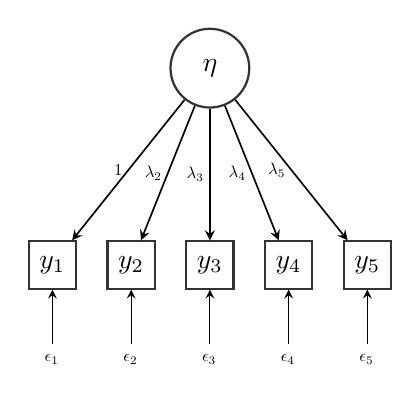
\begin{tikzpicture}[>=stealth,semithick]

% response variables
\node[ov] (y1) at (0,-1)      {$y_1$};
\node[ov] (y2) [right of=y1]  {$y_2$};
\node[ov] (y3) [right of=y2]  {$y_3$};
\node[ov] (y4) [right of=y3]  {$y_4$};
\node[ov] (y5) [right of=y4]  {$y_5$};

% error terms
\draw[thin, ->] (0, -2) -- (y1);
\draw[thin, ->] (1, -2) -- (y2);
\draw[thin, ->] (2, -2) -- (y3);
\draw[thin, ->] (3, -2) -- (y4);
\draw[thin, ->] (4, -2) -- (y5);
\node[text width=0cm, scale=0.6] at (-0.1, -2.2) {$\epsilon_1$};
\node[text width=0cm, scale=0.6] at (0.9, -2.2) {$\epsilon_2$};
\node[text width=0cm, scale=0.6] at (1.9, -2.2) {$\epsilon_3$};
\node[text width=0cm, scale=0.6] at (2.9, -2.2) {$\epsilon_4$};
\node[text width=0cm, scale=0.6] at (3.9, -2.2) {$\epsilon_5$};

% latent variable
\node[lv] (f1) at (2, 1.5)  {$\eta$};

% paths
\path[->] (f1) edge node[left,scale=0.6] {$1$} (y1)
          (f1) edge node[left,scale=0.6] {$\lambda_2$} (y2)
          (f1) edge node[left,scale=0.6] {$\lambda_3$} (y3)
          (f1) edge node[left,scale=0.6] {$\lambda_4$} (y4)
          (f1) edge node[left,scale=0.6] {$\lambda_5$} (y5);

\end{tikzpicture}


\end{document}
